% *******************************************************************************
% * Copyright (c) 2007 by Elexis
% * All rights reserved. This document and the accompanying materials
% * are made available under the terms of the Eclipse Public License v1.0
% * which accompanies this distribution, and is available at
% * http://www.eclipse.org/legal/epl-v10.html
% *
% * Contributors:
% *    G. Weirich - initial implementation
% *
% *  $Id: patneu.tex 2472 2007-06-03 09:48:14Z rgw_ch $
% *******************************************************************************
% !Mode:: "TeX:UTF-8" (encoding info for WinEdt)

Starten Sie Elexis durch Doppelklick auf das Programmsymbol.
Nach einem kurzen Moment erscheint ein Fenster etwa wie in Abb. \ref{fig:startbild} (sofern sie die
Demo-Datenbank verwenden, andernfalls sind die Fenster natürlich
leer).\footnote{Die Abbildungen dieser Tour entstammen Windows XP. Unter anderen Betriebssystemen wird das Aussehen leicht abweichend sein.}
 \begin{figure}[ht]
	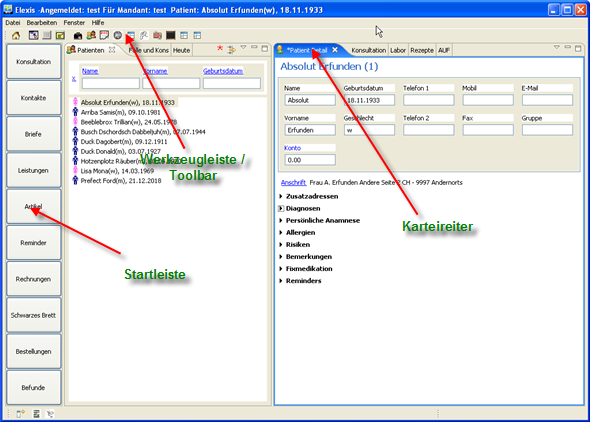
\includegraphics{images/einf0}
	\caption{Elexis Startbildschirm}
	\label{fig:startbild}
\end{figure}
\section{Patientendaten erfassen}
Aktivieren sie mit einem Klick die Ansicht 'Patienten' und schreiben Sie in die Eingabefelder Name und Vorname der neuen Patientin.
Falls die Patientin schon einmal erfasst worden ist erscheint ihr Name, in unserem Fall, wo keine Patientin dieses Namens vorhanden ist,
wird \glqq Keine Daten\grqq{}angezeigt (s. Abb. \ref{fig:patname}).
\begin{figure}[h]
	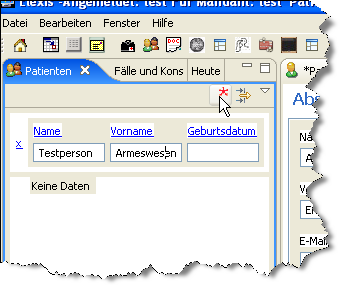
\includegraphics{images/einf1}
	\caption{Patientennamen eingeben}
	\label{fig:patname}
\end{figure}
Klicken Sie dann auf den roten Stern oben rechts, um eine Patientin mit diesen
Daten neu anzulegen. Es erscheint ein Dialogfenster (Abb. \ref{fig:patdata}), wo
Sie die Angaben in die entsprechenden Felder eingeben können.
\begin{figure}[ht]
	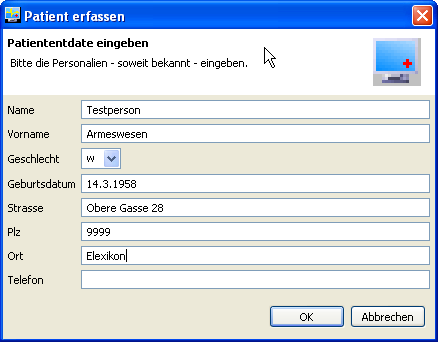
\includegraphics{images/einf2}
	\caption{Patientendaten ergänzen}
	\label{fig:patdata}
\end{figure}
Sie brauchen die hier verlangten Daten nicht vollständig einzugeben, sondern einfach soweit Sie diese im Moment kennen.
Sie müssen also im Notfalldienst nicht zuerst die vollständigen Daten eingeben, bevor Sie mit der Behandlung beginnen können.
Erfassen Sie z.B. nur Name und Geburtsdatum und überlassen Sie den Rest Ihrer MPA. Für Elexis ist ein neuer Patient in dem Moment bekannt,
wo Sie 'OK' klicken -- egal wieviele Daten zu diesem Zeitpunkt eingegeben sind.

\section{Falldaten erfassen}
Bei einer neuen Patientin müssen Sie zunächst einen \glqq Fall\grqq{} erstellen, dem
die Konsultation zugeordnet werden kann. Ein Fall sammelt alle Konsultationen, die einem gemeinsamen Garanten
zugeordnet werden können. Klicken Sie also in der \glqq Fälle\grqq{}-Ansicht
(Abb. \ref{fig:faelle}) auf den \glqq Neu\grqq{}-Stern.
\begin{figure}[ht]
	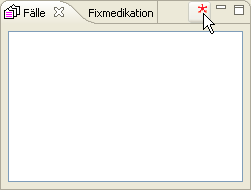
\includegraphics{images/einf3}
	\caption{Fälle-Ansicht}
	\label{fig:faelle}
\end{figure}
Dadurch öffnet sich ein Dialog, in dem Sie wiederum die Angaben eintragen
können, soweit diese Ihnen bekannt sind (Abb. \ref{fig:falldetail})
\begin{figure}[ht]
	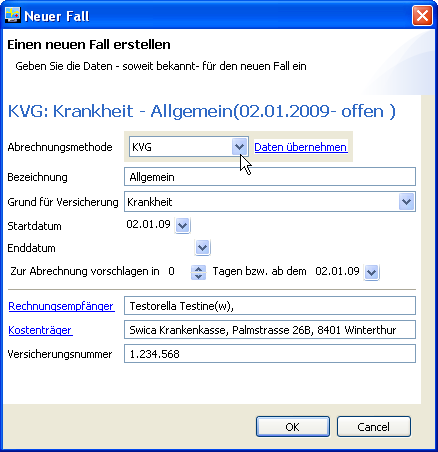
\includegraphics{images/einf4}
	\caption{Fall-Details}
	\label{fig:falldetail}
\end{figure}
Spätestens zur Rechnungsstellung müssen dann allerdings die notwendigen Angaben (Debitor, Kostenträger und Versicherungsnummer bzw. Fallnummer)
eingegeben werden.
Nach dem Klick auf OK haben Sie den neuen Fall erstellt. Bei weiteren
Konsultationen kann man sich diesen Schritt natürlich sparen.

Als nächstes erstellen wir eine neue Konsultation, wieder mit dem nun schon
bekannten Stern-Symbol (Abb. \ref{fig:neuekons}.
\begin{figure}[ht]
	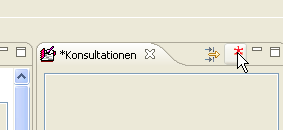
\includegraphics{images/einf5}
	\caption{Neue Konsultation}
	\label{fig:neuekons}
\end{figure}
\pagebreak[2]
Danach können wir mit dem KG-Eintrag beginnen (Abb. \ref{fig:KG}).
\section{Krankengeschichte führen}
\begin{figure}[ht]
	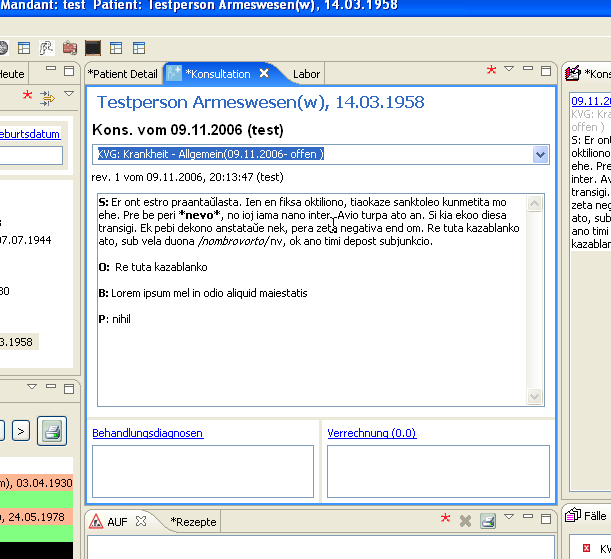
\includegraphics{images/einf6}
	\caption{KG-Eintrag}
	\label{fig:KG}
\end{figure}
Der KG-Eintrag kann einfache Textformatierungen enthalten, Textbausteine können
beliebig definiert und über eine konfigurierbare shortcut-Taste aufgerufen werden. Die Verrechnung erfolgt dann entweder über ein Tastaturmakro oder per Maus.
Nach Fertigstellung des Eintrags (auch vor oder während des Eintragens) können
Sie durch Klicken auf \glqq Verrechnung\grqq{} die Leistungen-Ansicht öffnen
(Abb. \ref{fig:Verrechnung}. Analog können sie durch klicken auf
\glqq Behandlungsdiagnosen\grqq{} die Diagnosen-Ansicht öffnen.\bigskip
\begin{figure}[ht]
	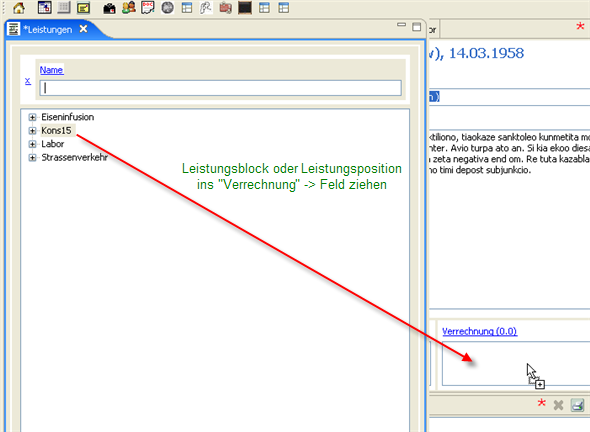
\includegraphics{images/einf7}
	\caption{Verrechnungs-Fenster}
	\label{fig:Verrechnung}
\end{figure}
Dieses Fenster enthält alle im System vorgesehenen Leistungscode-Systeme, sowie eine Seite mit selbstdefinierten Leistungsblöcken.
Sie können entweder einen ganzen Block oder einzelne Leistungen aus dem Block oder aus einem anderen Leistungsfenster (Tarmed etc.)
ins \glqq Verrechnung\grqq{}-Feld ziehen (drag an drop).

Genau gleich lassen sich zur Konsultation auch Diagnosen zuordnen, auch hier hat man die Wahl zwischen allen im System integrierten
Diagnosecodesystemen (beliebig anzupassen und erweiterbar).
\newpage{3}
Zum Abschluss möchten wir Ihnen noch zeigen, wie Sie eine View zur besseren Übersicht auf volle Bildgrösse und wieder
in ihren Originalzustand bringen können: Sie brauchen dazu nur auf dem Karteireiter der entsprechenden View doppelt zu
klicken (Abb. \ref{fig:viewmax}).
\begin{figure}[ht]
	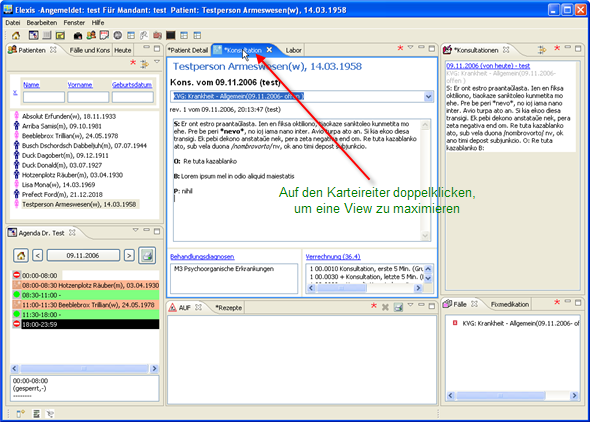
\includegraphics{images/einf8}
	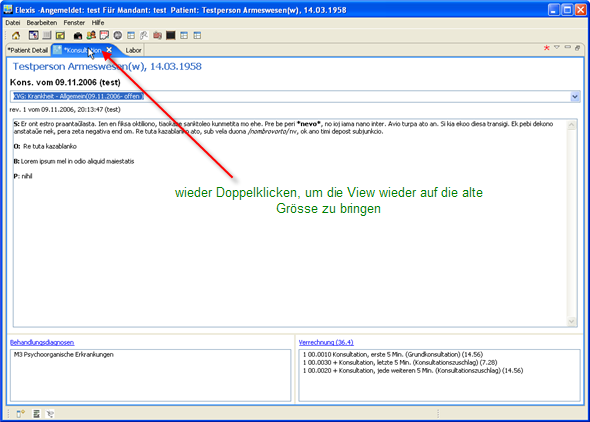
\includegraphics{images/einf9}
	\caption{View maximieren}
	\label{fig:viewmax}
\end{figure}

